\documentclass[12pt, twopage]{book}
\usepackage{lmodern}
\usepackage[T1]{fontenc}     % font encoding
\usepackage[utf8]{inputenc}  % input encoding
\usepackage{hyperref}        % hyperlinks
\usepackage{graphicx}
\usepackage[english]{babel}
\usepackage{mathtools}
\usepackage{stmaryrd}
\usepackage{amsfonts}
\usepackage{array}

\graphicspath{ {./images/} }
%%%%%%%%%%%%%%%%%%%%%%%%%%%%%%%%%%%%%%%%%%%%%%%%
% Chapter quote at the start of chapter        %
% Source: http://tex.stackexchange.com/a/53380 %
%%%%%%%%%%%%%%%%%%%%%%%%%%%%%%%%%%%%%%%%%%%%%%%%
\makeatletter
\renewcommand{\@chapapp}{}% Not necessary...
\newenvironment{chapquote}[2][2em]
{\setlength{\@tempdima}{#1}%
  \def\chapquote@author{#2}%
  \parshape 1 \@tempdima \dimexpr\textwidth-2\@tempdima\relax%
  \itshape}
{\par\normalfont\hfill--\ \chapquote@author\hspace*{\@tempdima}\par\bigskip}

\newcommand{\SEM}[1]{\llbracket #1 \rrbracket}


\title{
  \Huge \textbf{Bible}
  \\
  \huge {Proram Analysis}
}

\author{\textsc{Sangwoo Joh}\footnote{\url{https://sangwoo-joh.github.io}}}


\begin{document}

\frontmatter
\maketitle

\tableofcontents  % auto generate index from chapter, section, subsection, ...
\listoffigures  % auto generate list from figure's caption
\listoftables   % auto generate list from tagble's caption

\mainmatter


%%%%%%%%%%%%%%%%%%%%%%%%%%%%%%%%%%%%%%%%%%%%%%%%%%%%%%%%%%%%%%%%%%%%%%%%%
\chapter*{Preface}
This is personal bible, notes for everything I've learnt.


%%%%%%%%%%%%%%%%%%%%%%%%%%%%%%%%%%%%%%%%%%%%%%%%%%%%%%%%%%%%%%%%%%%%%%%%%%%%%%%%%%%%%%%%%%%%%%%%%%%
\chapter{Program Analysis}
\begin{chapquote}{H.G. Rice [1953], \textit{paraphrased by Anders Moller}}
  ``Everything interesting about the behaviour of programs is
  undecidable.''
\end{chapquote}

The goal of \textit{static program analysis} is to verify certain
\textsl{properties} (or \textsl{behaviours}, or
\textsl{specifications}, or \textsl{statements}, ...) of the target
program \textbf{without its execution}.

For program \textsl{P} and property \textsl{S},

\begin{itemize}
\item $ \SEM{P} $: Formal semantics of program \textsl{P}.

\item \textsl{S}: Semantic properties that we're interested in. This
  could be defined in various level, such as ``Division-by-zero will
  \textbf{never} occur'' or ``The variable \textit{i} is always 3''.

\item Soundness: $ analysis(P) = true \implies S $

\item Completeness: $ S \implies analysis(P) = true $

\item Scalability: Time complexity.
\end{itemize}


\textbf{No analysis} can be sound and complete at the same time. If an
analysis is sound, then it is also incomplete, and vice versa.


\section{Soundness}

It is called \textbf{sound} if an analysis for program \textsl{P} says
that it satisfies property \textsl{S}, then the program will truly
satisfy that property.

\textbf{Sound} but \textbf{incomplete} analysis have \textbf{false
  positive}. In other words, it does \textbf{not prove} programs that
satisfy the property.

\begin{figure}[h]
  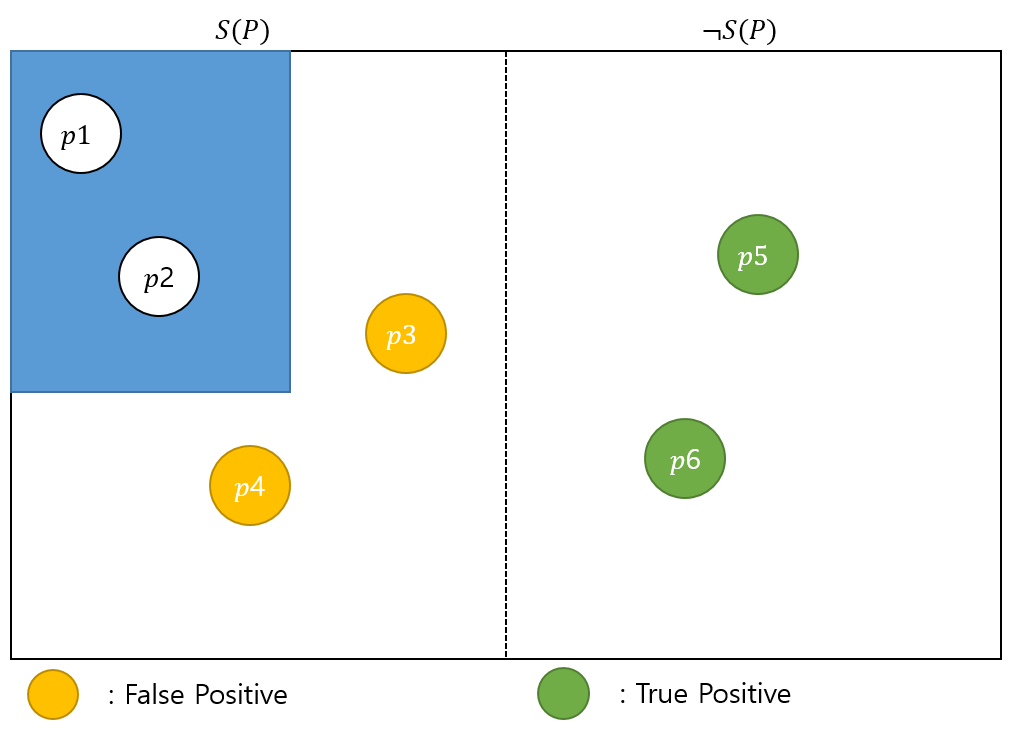
\includegraphics[width=\textwidth]{sound}
  \caption{Sound Analysis}
  \label{fig:sound}
\end{figure}

Figure \ref{fig:sound} shows a sound analysis (the blue area). It
proves correctly for the programs $ p_1 $ and $ p_2 $ that satisfy the
specification ($S(P)$). However, since this analysis is
\textit{incomplete}, it has \textbf{false positives}: it \textbf{does
  not prove} for programs $ p_3 $ and $ p_4 $ that satisfy $S$. In
other words, it proves that $ p_3 $ and $ p_4 $ satisfy $ \neg S(P) $
by emiting \textbf{alarms}, even though they are actually satisfy
$ S(P) $. False positives are also called as \textbf{false alarms}.


\section{Completeness}

An analysis is called \textbf{complete} when a program satisfies a
property \textsl{S}, the analysis for that program says that it will
satisfy that property.


\textbf{Complete} but \textbf{unsound} analysis have \textbf{false
  negative}. In other words, it \textbf{wrongly proves} programs that
does not satisfy the property.


\begin{figure}[h]
  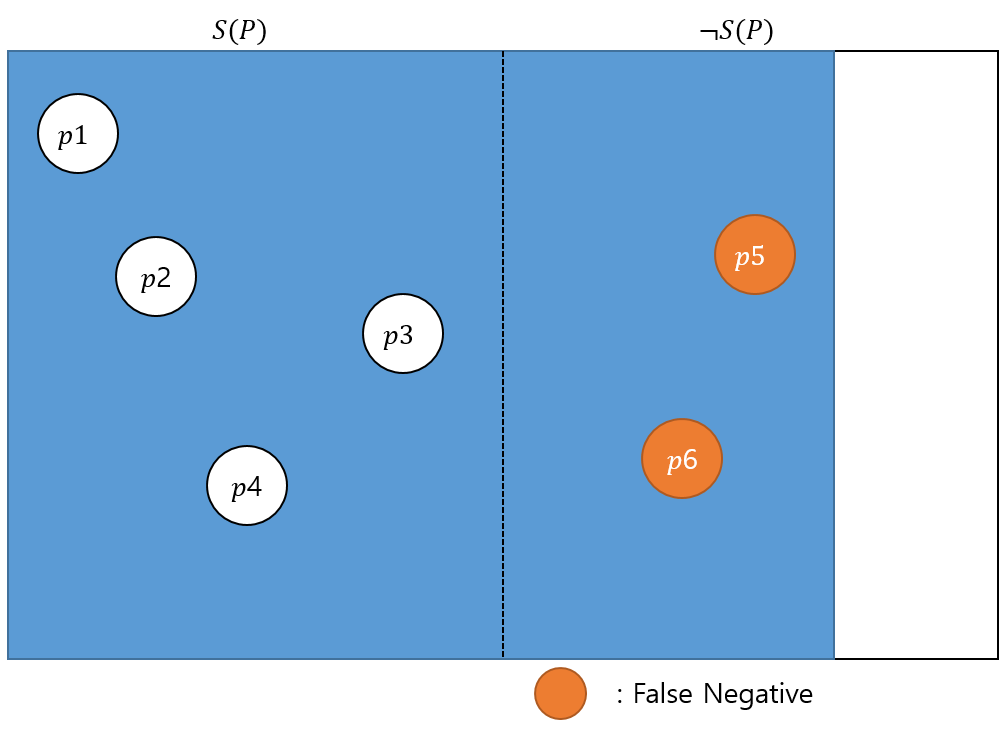
\includegraphics[width=\textwidth]{complete}
  \caption{Complete Analysis}
  \label{fig:complete}
\end{figure}

Figure \ref{fig:complete} shows a complete analysis (also the blue
area). It proves all the programs. In other words, it \textbf{wrongly
  proves} for programs $ p_5 $ and $ p_6 $ that actually do not
satisfy $ S(P) $ by accepting those programs (i.e., emitting no
alarms), thus it is \textit{unsound}. Those programs are \textbf{false
  negatives}.


The table \ref{tab:summary} shows the summary of soundness and
completeness.

\begin{table}[ht]
  \centering
  \caption{Sound \& Complete Summary}
  \label{tab:summary}

  \begin{tabular}[t]{l>{\raggedright}p{0.3\linewidth}>{\raggedright\arraybackslash}p{0.3\linewidth}}
    \hline
    & $ S(P) $ & $ \neg S(P) $ \\
    \hline
    Prove \texttt{(accept)} & \textbf{True negative} (\textsl{correct inference}) & False negative \\
    Not prove \texttt{(reject, alarm)} & False positive & \textbf{True positive} (\textsl{correct inference}) \\
    \hline
  \end{tabular}
\end{table}%



\section{Semantics}
\label{sec:semantics}

Semantics of the program defines the \textbf{meaning} of the program
that is grammatically correct.

\subsection{Operational Semantics}

Also called as \textit{transitional} semantics.

Semantics of a program is defined by the computation steps executed on
a machine. In other words, operational semantics is concerned about
\textbf{how to execute} the program and not merly what the execution
result is.

The semantics is defined as a transition system
$ ( \mathbb{S}, \to ) $, where

\begin{itemize}
\item $ \mathbb{S} $ is the set of all \textbf{possible states}.
\item $ \to \subseteq \mathbb{S} \times \mathbb{S} $ is a
  \textbf{transition relation} between two states. Describes how the
  execution takes place.
\item $ s \in \mathbb{S} $ is a \textbf{state} of the program, and is
  a pair $ ( l, m ) $ where $ l $ is a label and $ m $ is a machine
  state at that label during execution.
\end{itemize}

There are two approaches for operational semantics:

\begin{itemize}
\item \textsl{Big-step}: describes how the \textbf{overall results} of
  executions are obtained.
\item \textsl{Small-step}: describes how the \textbf{individual steps}
  of the computations take place.
\end{itemize}


The difference between the two are in the definitions of
\textsl{transition relation}.


\subsection{Denotational Semantics}
Also called as \textit{compositional} semantics.

Semantics of a program is defined by the semantics of the sub-parts of
the program. Thus, proving its soundness is by structural induction on
the program. For some realistic programming languages, even defining
their compositional semantics is an obstacle, due to \texttt{goto},
\texttt{exception}, or \texttt{call}.




%%%%%%%%%%%%%%%%%%%%%%%%%%%%%%%%%%%%%%%%%%%%%%%%%%%%%%%%%%%%%%%%%%%%%%%%%%%%%%%%%%%%%%%%%%%%%%%%%%%
\chapter{Abstract Interpretation}
\label{chap:ai}



\end{document}
